\documentclass{beamer}

\usepackage[french]{babel}
\usepackage[OT1]{fontenc}
\usepackage[utf8]{inputenc}

\definecolor{macouleur}{rgb}{.255,.243,.202}
\usecolortheme[named=macouleur]{structure}
\usetheme{AnnArbor}
\setbeamertemplate{blocks}[rounded, shadow=true]
\setbeamercolor{block title alert}{fg=white, bg=pink}

\title{Gestionnaire de rendez-vous}
\subtitle{Agenda electronique\\Outils utilisés : le  Langage C avec la bibliotheque SDL}
\institute[2017-2018]{Transmission des Données et Sécurité de l'Information}
\date{}
\author[L1TDSI]{Cheikh Tidiane Thiam\\Thierno Mamoudou Sabaly}

\begin{document}

\begin{frame}[t]
\includegraphics[scale=0.45]{Logolacgaa.png}
	\titlepage
\end{frame}

\begin{frame}[t]{INTRODUCTION}
Pour rappel, notre projet consiste à créer une application permettant de gerer les rendez-vous dans une clinique. En utilisant le langage C. A l'issu de notre présentation du projet et de la première soutenance, nous avions convenu de réaliser une application en fenêtre grace à la SDL.\pause \\Pour cette deuxième soutenance, notre présentation tournera autour de ces quatres points :\pause
\begin{enumerate}
\item \textcolor{blue}{Rappel sur la gestion des fichiers avec la console}\pause
\item \textcolor{blue}{Medecin-Secretaire et l'agenda électronique} \pause
\item \textcolor{blue}{Notion de Compte} \pause
\item \textcolor{blue}{Nuance sur la gestion des fichiers en console et en fenêtre} \pause
\end{enumerate}
\end{frame}

\begin{frame}{Console : Gestion de fichiers}
	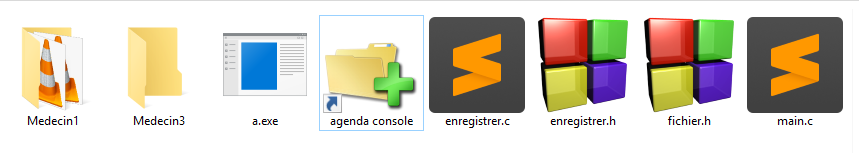
\includegraphics[scale = 0.5]{images/consolefile.PNG}
	 Console en arrière plan...
\end{frame}

\begin{frame}{Medecins-Secretaire et l'agenda electronique}
	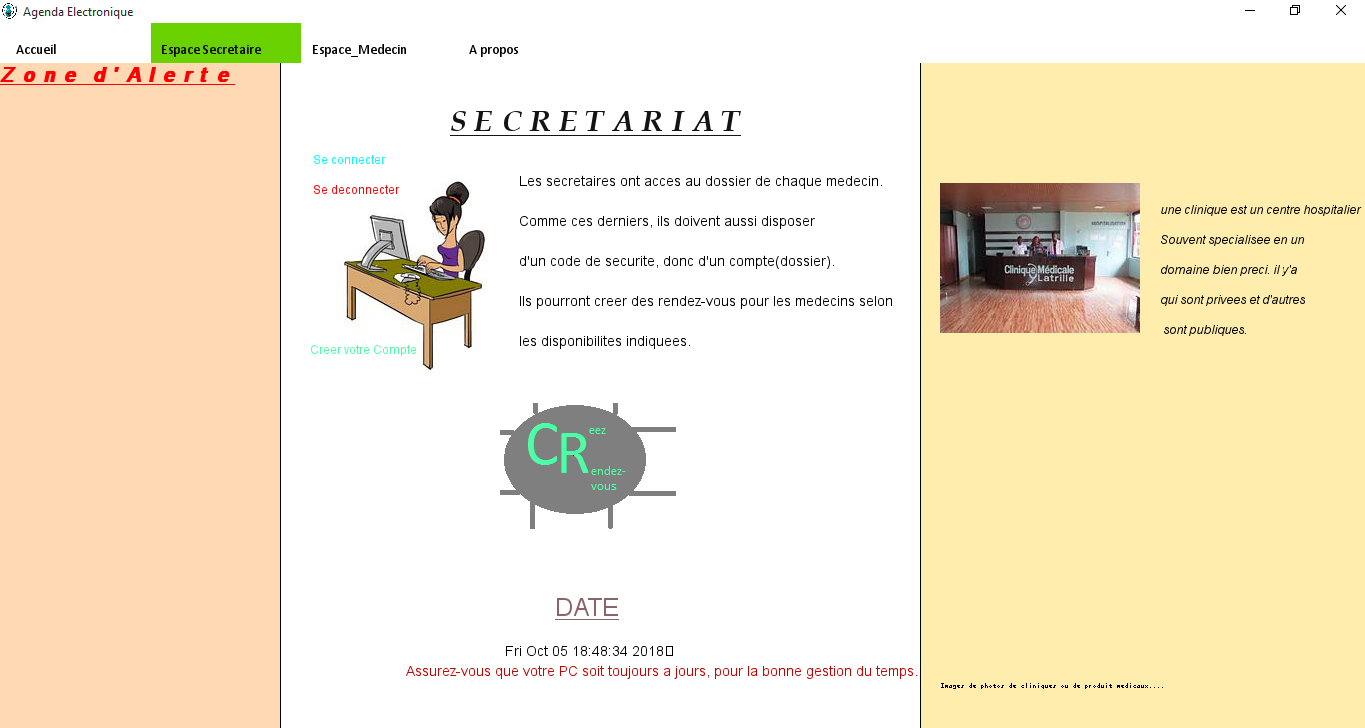
\includegraphics[scale = 0.30]{images/espacesec.PNG}
\end{frame}
\begin{frame}{Medecins-Secretaire et l'agenda electronique}
	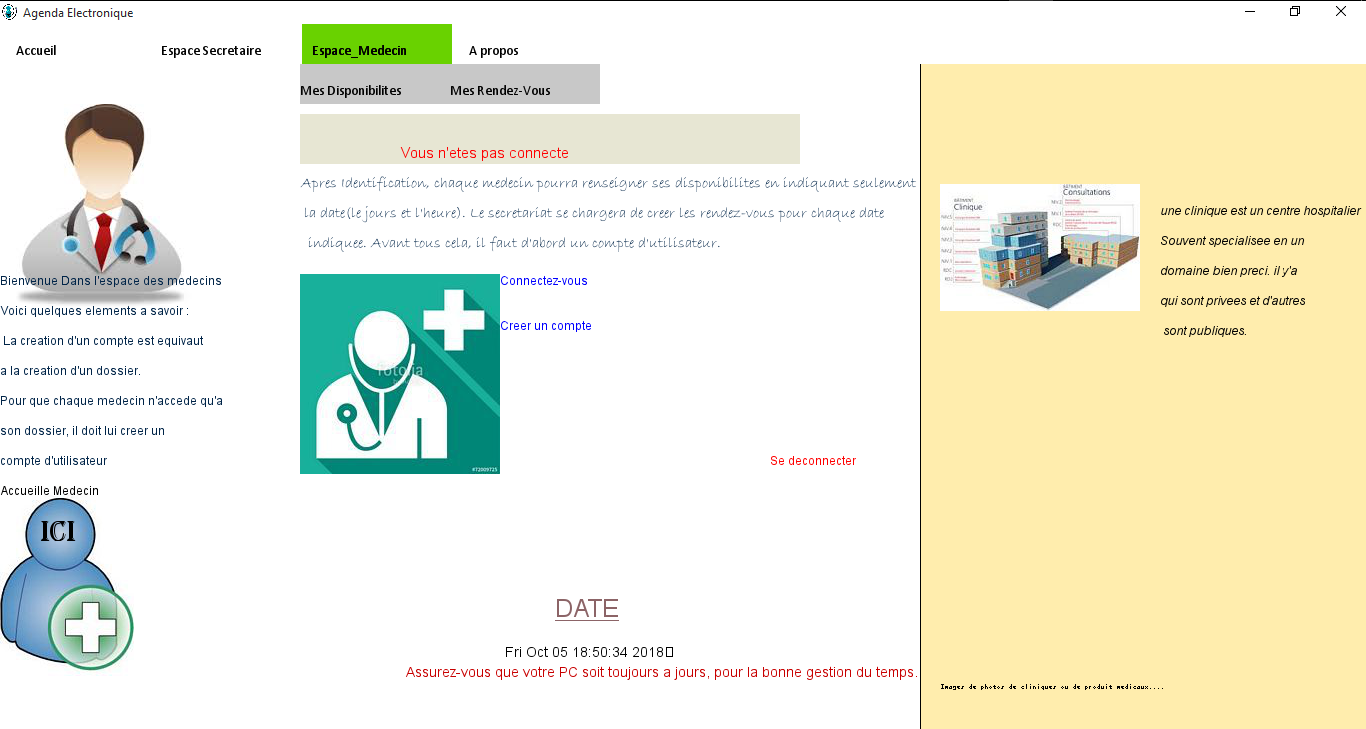
\includegraphics[scale = 0.30]{images/espacemed.PNG}
\end{frame}

\begin{frame}[t]{Notion  de Compte}\vspace{10pt}
	\textbf{Un compte en réalité c'est quoi?} \\ \pause
En faite nous avons cette relation :  \\  
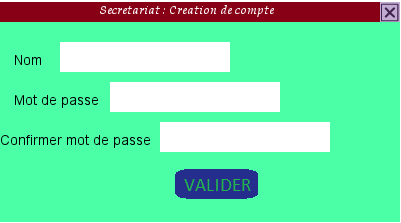
\includegraphics[scale = 0.45]{images/creecompte.PNG}   =  \pause

\includegraphics{images/fileopen.png}dossier actif\\ Creation d'un compte est égale à l'activation d'un dossier.\\ \pause
\textbf{Comment se passe cette activation?}
\end{frame}

\begin{frame}{Nuance sur la gestion des fichiers console et fenetre}
	 Dossier Principale \\ 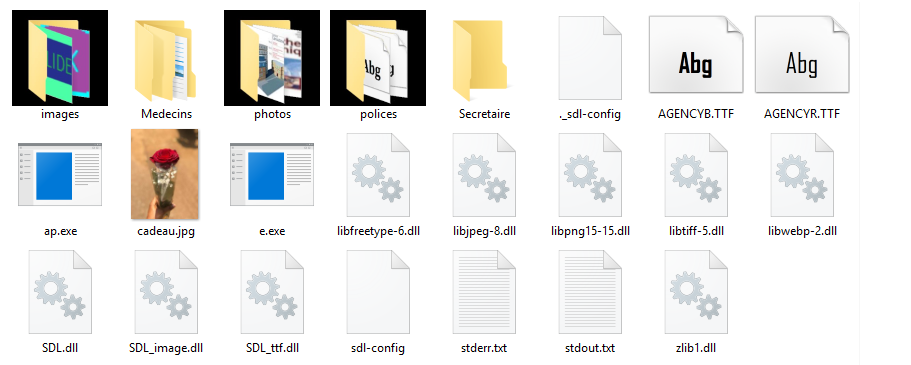
\includegraphics[scale = 0.45]{images/gestiondossier.PNG}
\end{frame}

\begin{frame}{Nuance sur la gestion des fichiers console et fenetre}
Dans le dossier Medecins\\ 
\includegraphics[scale = 0.5]{images/dossiermed.PNG} 
\end{frame}

\begin{frame}{Nuance sur la gestion des fichiers console et fenetre}
Le dossier d'un medecin\\ 
\includegraphics[scale = 0.5]{images/dansDmed.PNG} \\  
\end{frame}
\begin{frame}[t]{A venir}
Comme vous avez due le remarqué, Certaines disponibilités ont été enregistré dans le dossier du medecin ci-dessus. \pause En effet, désormais dans notre agenda  les médecins peuvent se connecter et renseigner leurs disponibilités, les visiter et entrer même
dans l'onglet dédié au rendez-vous. \pause Ces derniers seront bientôt disponibles car les sécretaire arrivent à se connecter. \\
\pause Il nous reste donc à réaliser la fonction permettant au sécrétaires d'acceder au dossiers des médecins.\\
Une fois l'enregistrement réglé, la suppression et la modification devient facile à réaliser. 
\end{frame}

\begin{frame}[t]{CONCLUSION}
\begin{block}{\textcolor{magenta}{Resume}}
	Nous insistons surtout sur la gestion des fichiers, parce que le fonctionnement de l'agenda electronique repose essentiellement sur une bonne gestion des fichiers. \\
Donc en résumé de  la même  façon pour la console, les rendez-vous créés seront sous forme de fichiers binaires classés soigneusement. On en fait de même pour les disponibilités des medecins.Tous ceci integrés à une fenetre, qui n'est autre qu'une décoration (dite "design"). L'agenda électronique est mi-fonctionnelle car l'onglet médecin est presque totalement active. Pour l'utiliser, medecin ou secretaire doit disposer d'un compte.Autrement dit, activer son dossier. \\ 
Nous concentrons notre travail sur la permission d'acces, pour la secretaire, au dossiers des medecins une fois connectée. Afin qu'elle puissse creer, supprimer ou modifier les rendez-vous des ces derniers.
\end{block}
\end{frame}
\end{document}